\documentclass[xcolor=table,10pt,final]{beamer}
\renewcommand\mathfamilydefault{\rmdefault}

\setbeamertemplate{navigation symbols}{}
\usepackage{amsmath,amsfonts,amssymb,pxfonts,xspace}
\usepackage{textcomp}
\usepackage{lmodern}
\usepackage{verbatim}
\usepackage{graphicx}
\usepackage{listings}
\usepackage[T1]{fontenc}

\lstset{
    basicstyle=\footnotesize,
    keywordstyle=\color[rgb]{0.1,0.8,0.1}\bfseries,
    commentstyle=\color{blue},
    numbers=left,
    stringstyle=\ttfamily\color{red!50!brown},
    showstringspaces=false}
\lstset{literate=%
   *{0}{{{\color{red!20!violet}0}}}1
    {1}{{{\color{red!20!violet}1}}}1
    {2}{{{\color{red!20!violet}2}}}1
    {3}{{{\color{red!20!violet}3}}}1
    {4}{{{\color{red!20!violet}4}}}1
    {5}{{{\color{red!20!violet}5}}}1
    {6}{{{\color{red!20!violet}6}}}1
    {7}{{{\color{red!20!violet}7}}}1
    {8}{{{\color{red!20!violet}8}}}1
    {9}{{{\color{red!20!violet}9}}}1
}



\begin{document}

\title{Python: beyond the basics}
\author{Albert DeFusco}
\date{\today}


\frame{\titlepage}

\begin{frame}[fragile]
  \frametitle{Review $\pi$}
  \begin{equation*}
    \pi = 2\prod^{\infty}_{i=1}\frac{4i^2}{4i^2-1}
  \end{equation*}
  \begin{itemize}
    \item<2-> How long to compute $\pi$ to 6 digits?\\
      \begin{lstlisting}[language=python]
from time import time
start=time()
#compute pi
print time()-start
      \end{lstlisting}
  \end{itemize}
\end{frame}

\begin{frame}[fragile]
  \frametitle{Functions and variables}
  \begin{itemize}
    \item Functions are defined in {\tt def} blocks\\
      \begin{lstlisting}[language=python]
def pi(i):
  """Compute the ith term of the Wallis formula"""
  return 4.*i**2 / (4.*i**2 - 1)

  print pi.__doc__
      \end{lstlisting}
    \item Multiple returns are tuples\\
      \begin{lstlisting}[language=python]
def myFunction(x,y):
  return x**2,y*4

a,b = myFunction(y=2,x=8)
      \end{lstlisting}
    \item Functions are objects
    \item Variables are passed by value
    \item Types are still implicit
    \item Global variables can be defined
      \begin{itemize}
        \item But not for passed variables
        \item Globals are not good OOP practice
      \end{itemize}
  \end{itemize}
\end{frame}

\begin{frame}[fragile]
  \frametitle{Functions and mutability}
  \begin{lstlisting}[language=python]
>>> def try_to_modify(x, y, z):
...     x = 23
...     y.append(42)
...     z = [99]
...     print(x)
...     print(y)
...     print(z)
...
>>> a = 77
>>> b = [99]
>>> c = [28]
>>> try_to_modify(a, b, c)
23
[99, 42]
[99]
>>> print(a)
77
>>> print(b)
[99, 42]
>>> print(c)
[28]
  \end{lstlisting}
\end{frame}

\begin{frame}[fragile]
  \frametitle{Numpy/Scipy Arrays}
  \begin{itemize}
    \item Homogeneous data types
    \item Contiguous memory layout
    \item Mathematical operations are much faster than lists
    \item Fixed length but mutable
    \item Multidimensional; row major
    \item For loops are slow
      \begin{itemize}
        \item Built-in operations make use of compiled code
        \item Array operations are auto-vectorized
      \end{itemize}
  \end{itemize}
  \vskip0.5cm
  \url{http://docs.scipy.org/doc/numpy/reference/index.html}
  \vskip0.5cm
  \begin{lstlisting}[language=python]
>>> import numpy as np
>>> help(np.<type/method>)
  \end{lstlisting}
\end{frame}


\begin{frame}[fragile]
  \frametitle{Array Creation}
  \lstinline[language=python]|import numpy as np|
  \begin{itemize}
    \item Manual\\
      \lstinline[language=python]|x = np.array([[1,2,3],[4,5,6]])|
    \item Creators
      \begin{itemize}
        \item Zero\\
          \lstinline[language=python]|np.zeros(N,M)|
        \item Ranges\\
          \lstinline[language=python]|np.arange(start,stop,increment)|\\
          \lstinline[language=python]|np.linspace(start,stop,n)|\\
          {\tt $\mathrm{start} <= x <= \mathrm{stop}$} for $n$ elements
        \item Identity\\
          \lstinline[language=python]|np.ones(N,M)|
        \item Unit diagonal\\
          \lstinline[language=python]|np.eye(N,M)|
        \item Diagonal\\
          \lstinline[language=python]|np.diag(<1d-array>)|
        \item Casting\\
          \lstinline[language=python]|np.array([i*0.5 for i in x])|
        \item Filling\\
          \lstinline[language=python]|a=np.empty((3,3));a.fill(42)|
        \item Tiling\\
          \lstinline[language=python]|a=np.tile(np.arange(0,3),(3,1))|

      \end{itemize}
  \end{itemize}
\end{frame}


\begin{frame}[fragile]
  \frametitle{Array types}
  \begin{itemize}
    \item The default is double precision\\
      \begin{lstlisting}[language=python]
>>> import numpy as np
>>> a = np.array([1,2,3])
>>> a.dtype
dtype('int64')
>>> a = np.array([1.,2.,3.])
>>> a.dtype
dtype('float64')
>>> a = np.ones(3,dtype=np.int32)
>>> a.dtype
dtype('int32')
      \end{lstlisting}
  \end{itemize}
\end{frame}


\begin{frame}
  \frametitle{Array Slicing}
  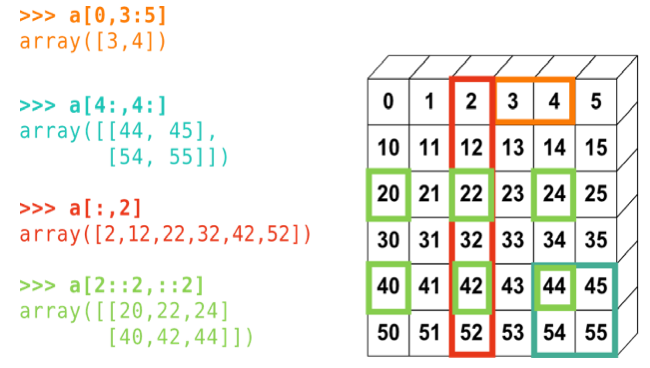
\includegraphics[width=.8\textwidth]{figures/slices}\\
  {\scriptsize \url{http://scipy-lectures.github.io/intro/numpy/array\_object.html\#indexing-and-slicing}}
\end{frame}

\begin{frame}[fragile]
  \frametitle{Array operations}
  \begin{itemize}
    \item Rshape\\
      \lstinline[language=python]|x.reshape(3,3)|
    \item Transpose\\
      \lstinline[language=python]|x.T|
    \item Elementwise operations\\
      \lstinline[language=python]|x**2|\\
      \lstinline[language=python]|x * y|\\
      \lstinline[language=python]|x + 1|\\
      \lstinline[language=python]|x > y|\\
      \lstinline[language=python]|np.sin(x)|
    \item Matrix multiplication\\
      \lstinline[language=python]|x.dot(y)|
    \item Masking creates copies\\
      \lstinline[language=python]|x[ x % 3 == 0 ]|\\
    \item Avoid loops
      \begin{itemize}
        \item The above operations are vectorized and very efficient
      \end{itemize}
  \end{itemize}
\end{frame}

\begin{frame}[fragile]
  \frametitle{Views}
  Slicing and other operations create a view, not a copy
\begin{lstlisting}[language=python]
> python
>>> import numpy as np
>>> x = np.array([[1.,2.],[3.,4.]])
>>> x
array([[ 1.,  2.],
       [ 3.,  4.]])
>>> y = x.T
>>> z = x.T.copy()
>>> y
array([[ 1.,  3.],
       [ 2.,  4.]])
>>> x[1] = 10.
>>> x
array([[  1.,   2.],
       [ 10.,  10.]])
>>> y
array([[  1.,  10.],
       [  2.,  10.]])
>>> z
array([[  1.,  2.],
       [  3.,  4.]])
\end{lstlisting}
\end{frame}

\begin{frame}[fragile]
  \frametitle{Arrays without loops}
  \begin{enumerate}
    \item Can you compute $\pi$ faster?
      \begin{itemize}
        \item Begin by reading {\tt pydoc numpy.lib}
        \item Can you do it without loops?
        \item I got a factor of 20 speed-up over last week's answer
      \end{itemize}
  \end{enumerate}
\end{frame}

\begin{frame}[fragile]
  \frametitle{Linear Algebra}
  {\tt pydoc scipy.linalg}
\end{frame}

\begin{frame}[fragile]
  \frametitle{Array exercises}
  \begin{enumerate}
    \item Devise a generic H\"{u}ckel solver for butadiene
      \begin{itemize}
        \item How would you build the matrix?
        \item How do you find the solution?\\
          $\alpha=0$ and $\beta = 1$\\
          \begin{equation*}
            \begin{bmatrix}
              \alpha - E & \beta & 0 & 0\\
              \beta & \alpha - E & \beta & 0\\
              0 & \beta & \alpha -E & \beta\\
              0 & 0 & \beta & \alpha -E\\
            \end{bmatrix}
          \end{equation*}
      \end{itemize}
  \end{enumerate}
\end{frame}


\begin{frame}
\end{frame}


\begin{frame}[fragile]
  \frametitle{Classes}
  \begin{lstlisting}[language=python]
  class Molecule(object):
    """Molecules have a name and chemical formula"""
    #Print the above message with "print <instance>.__doc__"
    weight=0
    def __init__(self,name)
      self.name = name
    def setName(self,name):
      self.name = name
    def setFormula(self,formula):
      self.formula=formula
    def computeWeight(self)
      try:
        weight = f(formula)
      except:
        print "the chemical formula was not set"
        return None
   \end{lstlisting}
   \begin{itemize}
     \item Private members and methods are name mangled
       \begin{itemize}
         \item \lstinline[language=python]|__name| becomes \lstinline[language=python]|_classname_name| at runtime
         \item Somewhat taboo in Python culture
       \end{itemize}
   \end{itemize}
\end{frame}

\end{document}
